%% For double-blind review submission
%\documentclass[sigplan,10pt,review,anonymous]{acmart}\settopmatter{printfolios=true}
%% For single-blind review submission
%\documentclass[sigplan,10pt,review]{acmart}\settopmatter{printfolios=true}
%% For final camera-ready submission
\documentclass[sigplan,10pt]{acmart}\settopmatter{}

%% Note: Authors migrating a paper from traditional SIGPLAN
%% proceedings format to PACMPL format should change 'sigplan' to
%% 'acmsmall'.


%% Some recommended packages.
\usepackage{booktabs}   %% For formal tables:
                        %% http://ctan.org/pkg/booktabs
\usepackage{subcaption} %% For complex figures with subfigures/subcaptions
                        %% http://ctan.org/pkg/subcaption


\makeatletter\if@ACM@journal\makeatother
%% Journal information (used by PACMPL format)
%% Supplied to authors by publisher for camera-ready submission
%\acmJournal{PACMPL}
\acmVolume{1}
\acmNumber{1}
\acmArticle{1}
\acmYear{2017}
\acmMonth{1}
\acmDOI{10.1145/nnnnnnn.nnnnnnn}
\startPage{1}
\else\makeatother
%% Conference information (used by SIGPLAN proceedings format)
%% Supplied to authors by publisher for camera-ready submission
\acmConference[FARM'17]{ACM SIGPLAN Workshop on Functional Art, Music, Modeling and Design}{September 9, 2017}{Oxford, UK}
\acmYear{2017}
\acmISBN{978-x-xxxx-xxxx-x/YY/MM}
\acmDOI{10.1145/nnnnnnn.nnnnnnn}
\startPage{1}
\fi


%% Copyright information
%% Supplied to authors (based on authors' rights management selection;
%% see authors.acm.org) by publisher for camera-ready submission
\setcopyright{none}             %% For review submission
%\setcopyright{acmcopyright}
%\setcopyright{acmlicensed}
%\setcopyright{rightsretained}
%\copyrightyear{2017}           %% If different from \acmYear


%% Bibliography style
\bibliographystyle{ACM-Reference-Format}
%% Citation style
%% Note: author/year citations are required for papers published as an
%% issue of PACMPL.
%\citestyle{acmauthoryear}  %% For author/year citations
%\citestyle{acmnumeric}     %% For numeric citations
%\setcitestyle{nosort}      %% With 'acmnumeric', to disable automatic
                            %% sorting of references within a single citation;
                            %% e.g., \cite{Smith99,Carpenter05,Baker12}
                            %% rendered as [14,5,2] rather than [2,5,14].
%\setcitesyle{nocompress}   %% With 'acmnumeric', to disable automatic
                            %% compression of sequential references within a
                            %% single citation;
                            %% e.g., \cite{Baker12,Baker14,Baker16}
                            %% rendered as [2,3,4] rather than [2-4].


\usepackage{balance}

\begin{document}

%% Title information
\title[]{FARM 2017 Demo Summary}         %% [Short Title] is optional;
                                        %% when present, will be used in
                                        %% header instead of Full Title.
%\titlenote{with title note}             %% \titlenote is optional;
                                        %% can be repeated if necessary;
                                        %% contents suppressed with 'anonymous'
%\subtitle{Subtitle}                     %% \subtitle is optional
%\subtitlenote{with subtitle note}       %% \subtitlenote is optional;
                                        %% can be repeated if necessary;
                                        %% contents suppressed with 'anonymous'


%% Author information
%% Contents and number of authors suppressed with 'anonymous'.
%% Each author should be introduced by \author, followed by
%% \authornote (optional), \orcid (optional), \affiliation, and
%% \email.
%% An author may have multiple affiliations and/or emails; repeat the
%% appropriate command.
%% Many elements are not rendered, but should be provided for metadata
%% extraction tools.

%% Author with single affiliation.
\author{Jean Bresson}
%\authornote{with author1 note}          %% \authornote is optional;
                                        %% can be repeated if necessary
%\orcid{nnnn-nnnn-nnnn-nnnn}             %% \orcid is optional
\affiliation{
  %\position{Position1}
  %\department{Department1}              %% \department is recommended
  \institution{UMR STMS: IRCAM/CNRS/UPMC Sorbonne Universit\'es}            %% \institution is required
%  \streetaddress{1, place Igor Stravinsky}
  \city{Paris}
%  \state{State1}
%  \postcode{Post-Code1}
  \country{France}
}
\email{jean.bresson@ircam.fr}          %% \email is recommended

%% Author with single affiliation.
\author{Michael Sperber}
%\authornote{with author1 note}          %% \authornote is optional;
                                        %% can be repeated if necessary
%\orcid{nnnn-nnnn-nnnn-nnnn}             %% \orcid is optional
\affiliation{
  %\position{Position1}
  %\department{Department1}              %% \department is recommended
  \institution{Active Group GmbH}            %% \institution is required
%  \streetaddress{1, place Igor Stravinsky}
  \city{T\"ubingen}
%  \state{State1}
%  \postcode{Post-Code1}
  \country{Germany}
}
\email{sperber@deinprogramm.de}          %% \email is recommended


%% Author with two affiliations and emails.
%\author{First2 Last2}
%\authornote{with author2 note}          %% \authornote is optional;
%                                        %% can be repeated if necessary
%\orcid{nnnn-nnnn-nnnn-nnnn}             %% \orcid is optional
%\affiliation{
%  \position{Position2a}
%  \department{Department2a}             %% \department is recommended
%  \institution{Institution2a}           %% \institution is required
%  \streetaddress{Street2a Address2a}
%  \city{City2a}
%  \state{State2a}
%  \postcode{Post-Code2a}
%  \country{Country2a}
%}
%\email{first2.last2@inst2a.com}         %% \email is recommended
%\affiliation{
%  \position{Position2b}
%  \department{Department2b}             %% \department is recommended
%  \institution{Institution2b}           %% \institution is required
%  \streetaddress{Street3b Address2b}
%  \city{City2b}
%  \state{State2b}
%  \postcode{Post-Code2b}
%  \country{Country2b}
%}
%\email{first2.last2@inst2b.org}         %% \email is recommended


%% Paper note
%% The \thanks command may be used to create a "paper note" ---
%% similar to a title note or an author note, but not explicitly
%% associated with a particular element.  It will appear immediately
%% above the permission/copyright statement.
%\thanks{with paper note}                %% \thanks is optional
                                        %% can be repeated if necesary
                                        %% contents suppressed with 'anonymous'


%% Abstract
%% Note: \begin{abstract}...\end{abstract} environment must come
%% before \maketitle command

\begin{abstract}
This is a summary of the demos presented at the 5th ACM SIGPLAN International Workshop on Functional Art, Music, Modelling and Design (FARM), prepared prior to the event. 
Extended abstracts of these demos are available on the FARM 2017 web site at \url{http://functional-art.org/2017/}.
\end{abstract}


%% 2012 ACM Computing Classification System (CSS) concepts
%% Generate at 'http://dl.acm.org/ccs/ccs.cfm'.
\begin{CCSXML}
<ccs2012>
<concept>
<concept_id>10011007.10011006.10011008.10011009.10011012</concept_id>
<concept_desc>Software and its engineering~Functional languages</concept_desc>
<concept_significance>500</concept_significance>
</concept>
<concept>
<concept_id>10010405.10010469</concept_id>
<concept_desc>Applied computing~Arts and humanities</concept_desc>
<concept_significance>500</concept_significance>
</concept>
%<concept>
%<concept_id>10011007.10011006.10011050.10011017</concept_id>
%<concept_desc>Software and its engineering~Domain specific languages</concept_desc>
%<concept_significance>300</concept_significance>
%</concept>
</ccs2012>
\end{CCSXML}

\ccsdesc[500]{Software and its engineering~Functional languages}
\ccsdesc[500]{Applied computing~Arts and humanities}
%\ccsdesc[300]{Software and its engineering~Domain specific languages}
%% End of generated code


%% Keywords
%% comma separated list
\keywords{functional programming, art, music, graphics, animation}  %% \keywords is optional


%% \maketitle
%% Note: \maketitle command must come after title commands, author
%% commands, abstract environment, Computing Classification System
%% environment and commands, and keywords command.
\maketitle



\section*{Introduction}

Six demonstrations were presented at the 5th ACM SIGPLAN International Workshop on Functional Art, Music, Modelling and Design (FARM). 
They range from applications of functional programming in music and sound, to more general purpose creative programming, and to 3D graphics and animation.
All extended abstracts are available on the FARM 2017 web site at \url{http://functional-art.org/2017/}.

%%% CHECK NUMBER OF PRESENTATIONS

\section{Representation of Musical Notation in Haskell}
%%% ASKED FOR MORE INFO
%%% ASKED FOR PICTURE

In this demonstration Edward Lilley (University of Cambridge, UK) introduces a formal computational approach to music notation. 
He illustrates his approach with computer representation of musical extracts using Haskell and an embedded Lilypond parser.
	


\section{The Arpeggigon: A Functional Reactive Musical Automaton}
%%% OK

Henrik Nilsson from the University of Nottingham (UK) presents the \textit{Arpeggigon}: 
an interactive cellular automaton for composing groove-based music. 
%
The \textit{Arpeggigon} is implemented in Haskell using the frameworks Functional Reactive Programming (FRP) and Reactive Values and Relations.
%
It is based on a hexagonal grid laid out as a harmonic table where each of the six possible directions corresponds to a given musical interval. 
%The automaton is configured by placing different types of tokens interacting on the grid, and runs by playing notes while some of these token perform moves on the grid.
The automaton is configured by placing different types of tokens on the grid: when the automaton is run, these tokens interact with one or more playheads moving around the grid, resulting in notes corresponding to the positions of the involved tokens to be played.
   
%\begin{figure}[h!]
%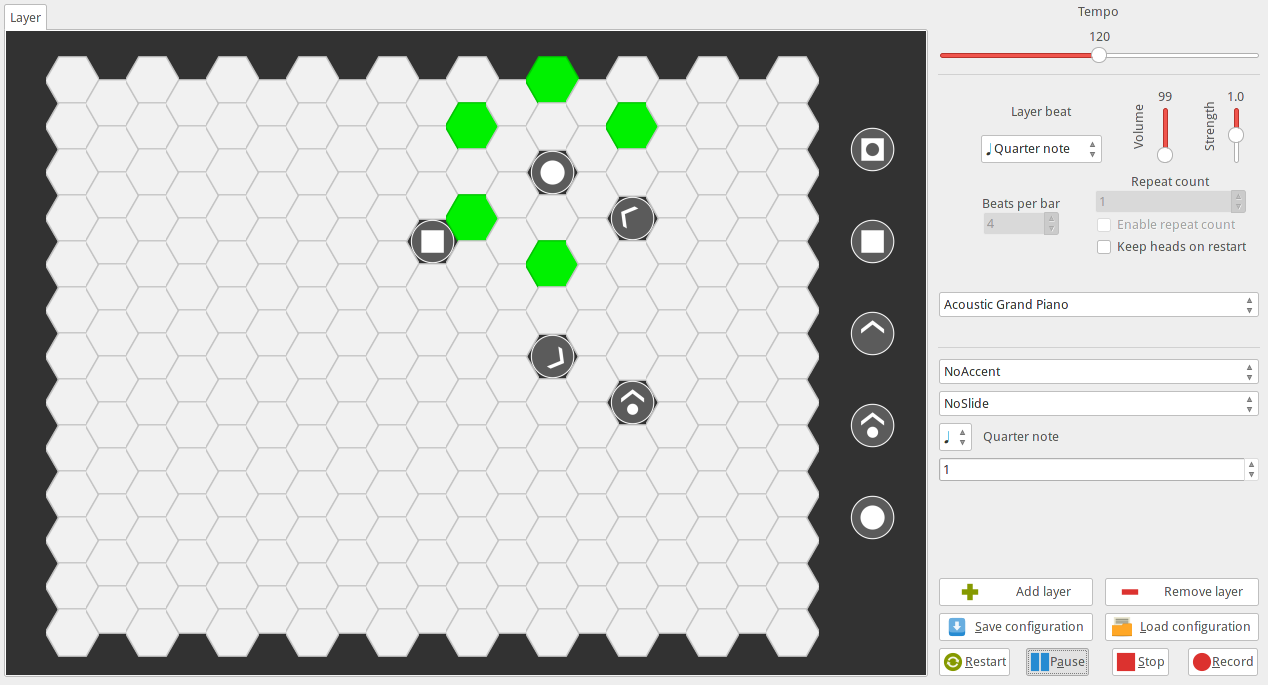
\includegraphics[width=.98\columnwidth]{./arpeggigon.png}
%\caption{\label{fig:octopus}
%The Arpeggigon by H. Nilsson.}
%\end{figure}


\section{Vivid: Sound Synthesis with Haskell and SuperCollider}
%%% ASKED FOR MORE INFO OR CONFIRMATION
%%% ASKED FOR PICTURE

Thomas Murphy (USA) presents a Haskell library for music creation and sound synthesis, coupled with the SuperCollider synthesis engine. 
\textit{Vivid} allows live-coding performance in Haskell, embedding advanced musical notions such as timing (at the musical and audio sample levels), parallelism, audio graphs, multichannel input and output, etc.


\section{African Polyphony and Polyrhythm}
%%% OK 
%%% NO PICTURE (?)

Chris Ford (ThoughtWorks, UK) proposes a programmatic approach to non-Western music analysis and representation, using functional programming to revisit ethnomusicologist Simha Arom's work and insights on Central African polyphony.
The demonstration takes examples notated in Arom's book \textit{African Polyphony and Polyrhythm}, and renders them in Lisp using the Leipzig composition library for Clojure. 



\section{Ait: A Concatenative Language for Creative Programming}
%%% ASKED FOR CONFIRMATION
%%% ASKED FOR PICTURE

Stian Veum M\o llersen (Bekk Consulting AS, Norway) presents the concatenative language \textit{Ait}. 
In concatenative languages, composing functions is implemented as the simple concatenation of words. I this presentation M\o llersen demonstrated how this programming style fits the idea of creative programming.
\textit{Ait} inherits the main features of previous concatenative languages such as Forth and Joy.
It is implemented in JavaScript with bindings to browser APIs, and therefore mainly targets web programming and applications.


%%%%%%%%%%%%%%%%%%%%%%%%%%%%%%%%%%%%%%%%%%%%%%%%%%%%%%%%%%%%%%%
%%%%%%%%%%%%%%%%%%%%%%%%%%%%%%%%%%%%%%%%%%%%%%%%%%%%%%%%%%%%%%%
%%%%%%%%%%%%%%%%%%%%%%%%%%%%%%%%%%%%%%%%%%%%%%%%%%%%%%%%%%%%%%%

\balance
\section{Octopus: A High-Level Fast 3D Animation Language}
%%% OK

David Janin and Simon Archipoff (LaBRI, University of Bordeaux, Bordeaux INP) complement a paper presentation on a new algebraic approach to media and 3D graphics programming that they developed, with this demonstration of the \textit{Octopus} language.
\textit{Octopus} is an EDSL (embedded domain-specific language) extending Haskell with an API for the definition of procedural 3D animations.
Conceptually the authors define their language as deriving from the classic LOGO with features extended to 3D graphics and animation (that is, including a time dimension). 
\textit{Octopus} programs generate small abstract drawing specifications on the CPU that are then sent to the OpenGL graphic pipeline for a fast expansion and rendering on the GPU.

%\begin{figure}[h!]
%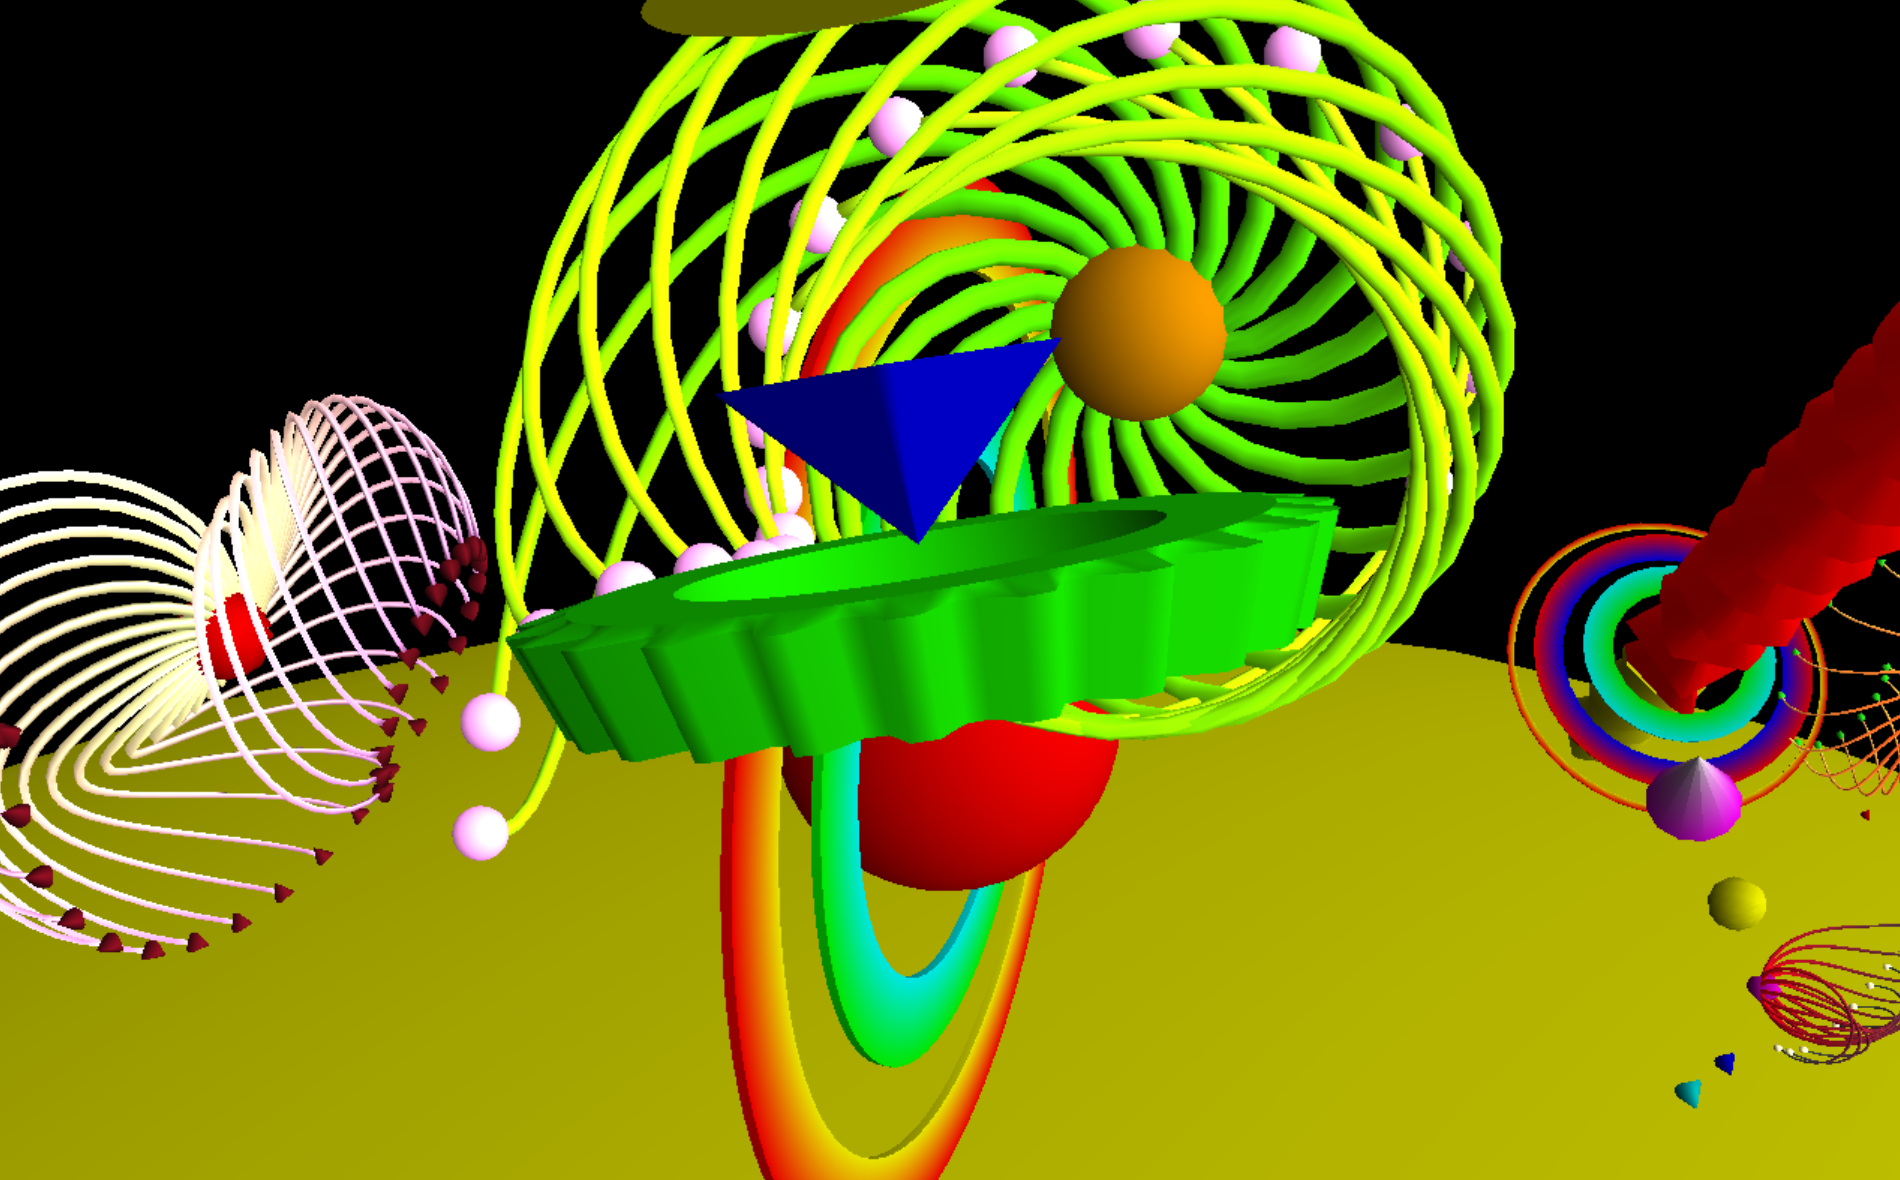
\includegraphics[width=.98\columnwidth]{./octopus.png}
%\caption{\label{fig:octopus}
%Octopus 3D animation rendering, by D. Janin and S. Archipoff.}
%\end{figure}

%%%%%%%%%%%%%%%%%%%%%%%%%%%%%%%%%%%%%%%%%%%%%%%%%%%%%%%%%%%%%%%
%%%%%%%%%%%%%%%%%%%%%%%%%%%%%%%%%%%%%%%%%%%%%%%%%%%%%%%%%%%%%%%
%%%%%%%%%%%%%%%%%%%%%%%%%%%%%%%%%%%%%%%%%%%%%%%%%%%%%%%%%%%%%%%

%\section{LambdaCube 3D: A Purely Functional DSL for Programming GPUs}
%Csaba Hruska and Andor P\'enzes	
%%% RESIGNED ?


%%% Acknowledgments
%\begin{acks}                            %% acks environment is optional
%                                        %% contents suppressed with 'anonymous'
%  %% Commands \grantsponsor{<sponsorID>}{<name>}{<url>} and
%  %% \grantnum[<url>]{<sponsorID>}{<number>} should be used to
%  %% acknowledge financial support and will be used by metadata
%  %% extraction tools.
%  This material is based upon work supported by the
%  \grantsponsor{GS100000001}{National Science
%    Foundation}{http://dx.doi.org/10.13039/100000001} under Grant
%  No.~\grantnum{GS100000001}{nnnnnnn} and Grant
%  No.~\grantnum{GS100000001}{mmmmmmm}.  Any opinions, findings, and
%  conclusions or recommendations expressed in this material are those
%  of the author and do not necessarily reflect the views of the
%  National Science Foundation.
%\end{acks}


%% Bibliography
%\bibliography{bibfile}


%% Appendix
%\appendix
%\section{Appendix}



\end{document}
